\chapter{Background \& Literature Review}
\label{chap2}
\label{background}

\begin{quote}
This chapter introduces the general context of the application of \emph{Probabalistic Graphical Models} in forecasting. The motivation of presenting this research is to \emph{accurately predict the behaviour of the energy markets} hence assist portfolio managers and energy traders in making better investment decisions. The application of  Probabilistic Graphical Models in making predictions has been discussed. Moreover, the \emph{macroeconomic structure of the oil markets} and the data sources from where the macroeconomic data is retrieved has also been discussed. Furthermore, the Python libraries being used for Bayesian Programming are also discussed.
\end{quote}


\section{Probabilistic Graphical Models}

Probablistic Graphical Models (PGMs) are a \emph{graphical} illustration of a \emph{joint probability distribution} which exploits dependencies between different \emph{random variables}. \\

PGMs allow us to describe the affect of one variable on the other and conversely, the independence of variables. The intersection of \emph{Graph Theory} and \emph{Probability Theory} allows us to construct better models that are not only better specified but also computationally more efficient. PGMs are essentially the outcome of giving a \emph{Graphical Structure} to variables of a probabilistic model and this process captures the relationships between variables and their uncertainties, conditional dependencies and independence.\\

There are two groups of Graphical Models: \emph{belief networks} and \emph{Markov networks}. The project would be applying both these Graphical Models as they are highly applicable in the construction of stochastic and probabilistic models of the energy markets. In this section, we would we introducing both these graphical models through definitions and examples and their applicability in making predictions in a general context. \\

\subsection{Belief Networks}

\textsc{Belief Networks} (also known as \emph{Bayesian Networks} or \emph{Bayesian Belief Networks}) are a way of illustrating the independence assumptions made in a probabilistic distribution. A belief network is primarily used to represent \emph{causal} relationships between random variables.\\

Causality is can be illustrated via trivial example\cite{cowell}. Suppose we attempt to switch on a computer, but we make an \emph{observation} that the computer does not switch on. We would like to know what could be the possible reasons of the failure. In a simplified model, we assume there are only \textbf{two} causes: \emph{electricity failure}, $E$, and \emph{computer malfunction}, $M$ to the observation of \emph{computer failure}, $C$. Below is an representation the \emph{graphical structure} of the causal model we have assumed.

\begin{figure}
\centering
\begin{tikzpicture}[
  								node distance=1.5cm and 0cm,
  								mynode/.style={draw,ellipse,text width=2.5cm,align=center}
							]
\node[mynode] (sp) {Electricity Failure};
\node[mynode,below right=of sp] (gw) {Computer Failure};
\node[mynode,above right=of gw] (ra) {Computer Malfunction};
\node[left=1.0cm of sp] (ali) {\textbf{Causes}};
\node[left=2.5cm of gw] (bob) {\textbf{Observations}};
\path (sp) edge[-latex] (gw)
(gw) edge[latex-] (ra);

\begin{pgfonlayer}{background}
\node[draw,inner sep=5pt,fill=gray!20,fit=(ra) (sp),rounded corners=4pt] (rect) {};
\end{pgfonlayer}

\begin{pgfonlayer}{background}
\node[draw,inner sep=5pt,fill=gray!20,fit=(gw),rounded corners=4pt] (rect) {};
\end{pgfonlayer}

\end{tikzpicture}
\caption{A graphical illustration of the structure of causal model.}
\end{figure}

\textbf{Bayes Theorem} allows us to calculate the conditional probability distribution of the \emph{unobserved causes} given the \emph{observed evidence}. \\

\vspace{-5mm}

\begin{frm-thm}[Bayes Theorem]

\textup{Given an \textup{unobserved cause} $H$ and \textup{observed evidence} $E$, the relationship between the \textcolor{blue}{posterior probability} \footnotemark, \textcolor{red}{likelihood} \footnotemark, \textcolor{darkgreen}{priori probability} \footnotemark, and \textcolor{magenta}{marginal probability} \footnotemark is given by: }

\begin{gather*}
\textcolor{blue}{P(H \mid E)} = \textcolor{red}{P(E \mid H)} \cdot \frac{\textcolor{darkgreen}{P(H)}}{\textcolor{magenta}{P(H)}}
\end{gather*}


\end{frm-thm}


\footnotetext[1]{\emph{Posterior} probability is the probability of the \emph{unobserved cause} \emph{after} knowing the \emph{observed evidence}.}
\footnotetext[2]{\textit{Likelihood} is the probability of the \emph{unobserved evidence} given the \emph{observed cause}.}
\footnotetext[3]{\emph{Priori} probability is the probability of the \emph{unobserved cause} \emph{before} knowing the \emph{observed evidence}.}
\footnotetext[4]{\emph{Marginal} probability is the \emph{total} probability of the \emph{observed evidence}.}

Refering back to our example of from Cowell \cite{cowell}, we can see the the \emph{causes} are 'electricity failure' and 'computer malfunction', whereas the \emph{observations} are 'computer failure'. Assume that '$E$ occurs with probability $P(E = true) = 0.1$, and $M$, occurs with probability $P(M = true) = 0.2$. Also assume that the property $P(E, M) = P(E) \cdot P(M)$ holds (i.e. $E$ and $M$ are independent).  Also assume (for the sake of \emph{simplicity}) that the if there is no problem with electricity and the computer has no malfunction, then $P(C = true \mid E = false, M = false)$. Lastly, we assume that if there is an electricity malfunction, the computer will not start regardless the if there is a computer malfunction, i.e. $P(C = true \mid E = true, M = false) = 1$ and $P(C = true \mid E = true, M = true) = 1$. Given these assumptions, we can calculate the the \emph{priori} probability $P(C = true)$ using \emph{marginalisation} \cite{barberBRML2011}.

\begin{equation*}
\begin{aligned}
P[C = true] ={} & \sum_{E, M}^{} P[C = true, E, M] \\
				  ={} & \sum_{E, M}^{} P[C = true \mid E, M] \cdot P[E] \cdot P[M] = \textbf{0.19}
\end{aligned}
\end{equation*}

Now, using this result, we can draw conculsions on the \emph{unobserved causes} given the \emph{observed evidence}. For example, if we try to switch on the computer but it does not start, we can calculate the probability distribution of the \emph{unobserved causes} \textbf{given} the \emph{observed evidence}.\\

For calculating the probability that there has been an electricity failure (\emph{unobserved cause}) \textbf{given} the computer is not switching on,

\begin{equation*}
\begin{aligned}
P[E = true \mid C = true] ={} & \sum_{M} P[E = true, M \mid C = true] && \textbf{Marginalisation}  \\
       								  ={} & \sum_{M} \frac{P[C = true \mid E = true, M] \cdot P[E = true] \cdot P[M]}{P[C = true]} && \textbf{Bayes' Theorem} \\
       								  ={} & \frac{1 \cdot 0.1 \cdot 0.2}{0.19} +\frac{1 \cdot 0.1 \cdot 0.8}{0.19} = \frac{10}{19} \approx \textbf{0.53}
\end{aligned}
\end{equation*}

For calculating the probability that there has been an computer malfunction (\emph{unobserved cause}) \textbf{given} the computer is not switching on,

\begin{equation*}
\begin{aligned}
P[M = true \mid C = true] ={} & \sum_{E} P[E, M = true \mid C = true] && \textbf{Marginalisation}  \\
                                           ={} & \sum_{E} \frac{P[C = true \mid E, M = true] \cdot P[E] \cdot P[M = true]}{P[C = true]}  && \textbf{Bayes' Theorem} \\
                                           ={} & \frac{1 \cdot 0.1 \cdot 0.2}{0.19} +\frac{0.5 \cdot 0.9 \cdot 0.2}{0.19} = \frac{11}{19} \approx \textbf{0.58}
\end{aligned}
\end{equation*}

\textbf{Belief Networks} heavily rely on \emph{Bayes' Theorem} for calculating \emph{joint probability distributions} of variables using \emph{conditional probabilities} obtained from \emph{Bayes' Theorem} .

\begin{frm-def}[Belief Network ]
\textup{A Belief Network is a \emph{directed acyclic graph} $G = \braket{V,E}$ where every vertex $v \in V$ is associated with a random variable $X_v$, and every edge $(u,v) \in E$ represents a direct dependence from a random variable $X_u$ to a random variable $X_v$ \cite{Gordon-2014}. The probability distribution function is of the form\cite{barberBRML2011}:}
\vspace{-3mm}
\begin{gather*}
p(x_1, \cdots, x_D) = \prod_{i=1}^{D} p(x_i \mid \textup{pa} (x_i))
\end{gather*}
\textup{where $\textup{pa}(x_i)$ represents the parental variables of $x_i$, and the $i^{th}$ vertex in the graph corresponding with the factor $p(x_i \mid \textup{pa} (x_i))$ \footnotemark. In a belief Network, each node $v \in V$ corresponds to a \emph{Conditional Probability Table}, \textsf{CPD}$(v)$, which denotes the probability distribution of $X_v$, conditioned over the values of the random variables associated with the direct dependencies $D(v) = \{u \mid (u,v) \in E\}$.}

\end{frm-def}

\footnotetext[1]{In the case of a random variable having no parents, $p(x_i \mid \textup{pa} (x_i)) = p(x_i)$.}

\vspace{-3mm}

In order to explain the concept of belief networks better, the most common example that is given is that of the "Rain-Sprinkler-Wet Grass" model, which is popularly described in literature in Statistics and Machine Learning.

\vspace{3mm}

\begin{figure}
\begin{tikzpicture}[
  node distance=1cm and 0cm,
  mynode/.style={draw,ellipse,text width=2cm,align=center}
]
\node[mynode] (sp) {Sprinkler};
\node[mynode,below right=of sp] (gw) {Grass wet};
\node[mynode,above right=of gw] (ra) {Rain};
\path (ra) edge[-latex] (sp)
(sp) edge[-latex] (gw)
(gw) edge[latex-] (ra);
\node[left=0.5cm of sp]
{
\begin{tabular}{cM{2}M{2}}
\toprule
& \multicolumn{2}{c}{Sprinkler} \\
Rain & \multicolumn{1}{c}{T} & \multicolumn{1}{c}{F} \\
\cmidrule(r){1-1}\cmidrule(l){2-3}
F & 0.4 & 0.6 \\
T & 0.01 & 0.99 \\
\bottomrule
\end{tabular}
};
\node[right=0.5cm of ra]
{
\begin{tabular}{M{1}M{1}}
\toprule
\multicolumn{2}{c}{Rain} \\
\multicolumn{1}{c}{T} & \multicolumn{1}{c}{F} \\
\cmidrule{1-2}
0.2 & 0.8 \\
\bottomrule
\end{tabular}
};
\node[below=0.5cm of gw]
{
\begin{tabular}{ccM{2}M{2}}
\toprule
& & \multicolumn{2}{c}{Grass wet} \\
\multicolumn{2}{l}{Sprinkler rain} & \multicolumn{1}{c}{T} & \multicolumn{1}{c}{F} \\
\cmidrule(r){1-2}\cmidrule(l){3-4}
F & F & 0.4 & 0.6 \\
F & T & 0.01 & 0.99 \\
T & F & 0.01 & 0.99 \\
T & T & 0.01 & 0.99 \\
\bottomrule
\end{tabular}
};

\end{tikzpicture}
\caption{The 'Rain-Sprinkler-Wet Grass' belief network example.}
\end{figure}


In this model, we can use the \emph{observed evidence} of the grass being wet to calculate the probabilities of the \emph{unobserved causes}. For example, we can calculate the probability of the sprinkler being on (\emph{evidence}) given the grass is wet (\emph{observation}). \\

\vspace{-5mm}

\begin{equation*}
\begin{aligned}
P[R = T \mid G = T] ={} & \frac{P[G = T, R = T]}{P[G = T]} && \textbf{Bayes' Theorem} \\[3mm]
							  ={} & \frac{\sum_{S} P[G = T, S, R = T]}{\sum_{S,R} P[G = T, S, R]} && \textbf{Marginalisation} \\[3mm]
\end{aligned}
\end{equation*}

\begin{equation*}
\begin{aligned}
\sum_{S} P[G = T, S, R = T] ={} &  P[G = T, S = T, R = T] \hspace{2mm} +  \\
										  ={} &  P[G = T, S = F, R = T] \\
							 			  ={} & P[G = T \mid S = T, R = T] \cdot P[S = T \mid R = T] \cdot P[R = T ]  \hspace{2mm}+ \\
							 			    {} & P[G = T \mid S = F, R = T] \cdot P[S = F \mid R = T] \cdot P[R = T] && \textbf{Joint P.D.F} \\
							 			  ={} & 0.01 \cdot 0.01 \cdot 0.2 + 0.01 \cdot 0.99 \cdot 0.2
							 			  ={} \textbf{0.002}
\end{aligned}
\end{equation*}

\begin{equation*}
\begin{aligned}
\sum_{S} P[G = T, S, R] ={} &  P[G = T, S = T, R = T] \hspace{2mm} \hspace{2mm} + \\
									  {} &  P[G = T, S = T, R = F] \hspace{2mm} \hspace{2mm} + \\
									  {} &  P[G = T, S = F, R = T] \hspace{2mm} \hspace{2mm} + \\
									  {} &  P[G = F, S = F, R = F] \hspace{2mm} \hspace{2mm} + \\[2mm]
							 	    ={} & P[G = T \mid S = T, R = T] \cdot P[S = T \mid R = T] \cdot P[R = T ]  \hspace{2mm}+ \\
							 	    	  {} & P[G = T \mid S = T, R = F] \cdot P[S = T \mid R = F] \cdot P[R = F ]  \hspace{2mm}+ \\
							 	      {} & P[G = T \mid S = F, R = T] \cdot P[S = F \mid R = T] \cdot P[R = T ]  \hspace{2mm}+ \\
							 		  {} & P[G = T \mid S = F, R = F] \cdot P[S = F \mid R = F] \cdot P[R = F] && \textbf{Joint P.D.F} \\[2mm]
							 	    ={} & 0.01 \cdot 0.01 \cdot 0.2 + 0.01 \cdot 0.99 \cdot 0.2 + 0.01 \cdot 0.4 \cdot 0.8 + 0.4 \cdot 0.6 \cdot 0.8 \\
							 	    ={} & \textbf{0.1972}
\end{aligned}
\end{equation*}

\begin{equation*}
\begin{aligned}
\therefore P[R = T \mid G = T] ={} & \frac{\sum_{S} P[G = T, S, R = T]}{\sum_{S,R} P[G = T, S, R]} \\
							  ={} & \frac{0.002}{0.1972} \approx 0.01
\end{aligned}
\end{equation*}

Therefore the probability that \emph{it is raining}, \textbf{given} that the grass is wet, is \textbf{1\%}.\\

In the next section, we would be exploring different algorithms used to learn and construct belief networks. Learning belief networks plays a very important role as it enables us to perform \textit{inferences} on the model and obtain valuable forecasts.

\subsubsection{Learning Belief Networks}
\label{learn}

The sections demonstrate how belief networks represent a probability distribution over a set of variables, and how they can be used e.g. to predict variable states, or to generate new samples from the joint distribution. This section concerns on the process of obtaining a belief network, given a set of sample data. Learning a belief network can be split into two problems:\\

\begin{description}
	\item[Parameter learning:]{Given a set of data samples and a DAG (Directed Acyclic Graph) that captures the dependencies between the variables, estimate the conditional probability distributions of the individual variables. Each factor is a conditional density depending on a restricted number of parameters which we can often estimate separately.}
	\item[Structure learning:]{Given a set of data samples, estimate a DAG that captures the dependencies between the variables. This step determines which arcs are in the graph without looking at parameter estimates.}
\end{description}

Most of academic literature focuses on structure learning which is the most challenging part. Indeed, the problem is certainly computationally expensive and a naive brute-force approach (greedy search) will usually does not work. In what follows, we will describe the general framework of learning belief networks and present a general overview of two algorithms that can be used more specifically for structure learning.

\paragraph{Parameter learning}

Let us assume that a graph $G$ has been selected and we have a parametric model $p(x_V;\theta)$, such that for each node $v \in V$, we can associate a subset of the parameters $\theta_{v\mid\text{pa}(v)}\subset \theta$ and express the conditional density of $v$ given its parents,

\begin{eqnarray*}
p_{v\mid \text{pa}(v)}(x_{v};\theta) &=& p_{v\mid \text{pa}(v)}(x_v;\theta_{v\mid \text{pa}(v)}).
\end{eqnarray*}

One of the major advatanges of using a graphical model is that the estimation problem is reduced to a set of lower dimension problems. The parameter learning step is computational feasible, assuming that $\theta_{v\mid \text{pa}(v)}$, $v\in V$ form a partition of $\theta$.  However, often it is enough to estimate the parameter $\theta_v$ in each component $p_{v\mid \text{pa}(v)}(x_{v\mid \text{pa}(v)}\mid \theta_{v\mid \text{pa}(v)})$ separately, which could be done by standard estimators such as \hyperref[mle]{maximum likelihood estimator}.\\

We can observe that the sparser the graph $G$ is, the smaller the expected dimension of parameters $\theta_{v\mid \text{pa}(v)}$, and therefore we can conclude that there is a computational incentive to select sparser graphs. We can also observe that issues arise when the sample size is smaller than the number of variables, which tends to increase the variability of data. This problem is frequently faced in Computational biology when the number of observations ends up smaller than the number of genes.\\

Parameter learning is for \textit{discrete} nodes is of two main types:

\begin{description}
		\item[Maximum Likelihood Estimation:]{\label{mlw} A natural estimate for the CPDs is to simply use the relative frequencies, with which the variable states have occured. According to MLE, we should fill the CPDs such that $P(\text{data}|\text{model})$ is maximised. This is achieved when using the relative frequencies\cite{875348}.}
		\item[Bayesian Estimation:]{The Bayesian Parameter estimator begins with already existing prior conditional probability tables that express our beliefs about the variables before the data was observed. }
\end{description}

\paragraph{Structure learning}
\label{structure}

It is well known in the literature that the problem of learning the structure of belief is very challenging one to tackle: given computational complexity can often become super-exponential in the number of nodes in the worst case and polynomial in most real-world scenarios.\\

Structure learning is process of finding a directed acyclic graph (DAG) $G = \braket{V, E}$ that maximises $\mathbb P(G\mid D)$, and we can express the quantity as follows:

\begin{eqnarray*}
\mathbb P(\mathcal G\mid D)
&\propto\,\, \mathbb P(\mathcal G)\,\mathbb P(D\mid \mathcal G)
\end{eqnarray*}

In context of Bayesian statistics, we could begin with selecting a prior $\mathbb P(\mathcal G)$ over all possible DAGs\cite{castelo2000priors}. In practice this is somewhat challenging since the set of all possible graphs grows super exponentially to the number of variables in the network. Without having any prior knowledge on the graph structure, it is commonplace to use the following uniform prior: for every pair $(i, j) \in V$, we assign:

\begin{itemize}
	\item{An edge $i \to j$ with probability $p_\ell=1/4$, or}
	\item{An edge $j \to i$ with probability $p_r =1/4$, or}
	\item{No arc between $i$ and $j$ with probability $p_0 = 1/2$}
\end{itemize}

Another possibility is to assign all the three options with equal probability $p = 1/3$. Often in literature, a uniform prior is implicitly assumed with $P(\mathcal G\,|\, D)\propto \mathbb P(D\,|\, \mathcal G)$.

\subparagraph{Constraint-based learning}

\label{constraint}

This class of algorithm \cite{scutari2014bayesian} uses conditional independence tests to determine which arcs belong to the graph. Note that for that , we do not need to assume conditional independence in probability implies conditional independence on the graph so that $\perp\!\!\perp_p \Leftrightarrow \perp\!\!\perp_{G}$. Compared to the basic case, this is a stricter set of assumptions than the basic case where we assume $\perp\!\!\perp_G \Rightarrow \perp\!\!\perp_p$. The most popularly used independence tests are Pearson's $\chi^2$-test for categorical data, the exact $t$-test for Pearson's correlation coefficient (for Gaussian data), and Fisher's $Z$-test (for Gaussian data).\\

All constraint-based learning algorithms share a common three-phase structure as illustrated in the Inferred Causation algorithm. The first phase consists of learning the \hyperref[blanky]{Markov blanket} of each node to reduce the number of candidate DAGs early on. The second phase involves learning the skeleton of the DAG, that is, it identifies which undirected arcs are present in the DAG. Finally, in the third step, the arc directions are established and a complete partially directed acylic graph is returned. \\

Before explaining the \hyperref[icalgo]{inferred causality} algorithm, let us revise what \hyperref[blanky]{Markov blankets} are and their role in graphical models.

\begin{figure}
\label{blanky}
\centering
    \begin{tikzpicture}[font=\sffamily]

        \node[state]    (state1)  {$v$};
        \node[state, fill=blue, above=10mm of state1, text opacity=0]    (state2)  {$s$};
        \node[state, fill=blue, above left=10mm and 7mm of state1, text opacity=0]    (state3)  {$s$};
        \node[state, fill=blue, above right=10mm and 7mm of state1, text opacity=0]    (state4)  {$s$};
        \node[state,fill=green, below left=10mm and 7mm of state1, text opacity=0]    (state5)  {$s$};
        \node[state,fill=green, below right=10mm and 7mm of state1, text opacity=0]    (state6)  {$s$};
        \node[state,above left=10mm and 3mm of state3, text opacity=0]    (state7)  {$s$};
        \node[state,below left=13mm and 2mm of state7, text opacity=0]    (state8)  {$s$};
         \node[state,left=20mm of state1, text opacity=0]    (state9)  {$s$};

         \node[state,above right=13mm and 7mm of state4, text opacity=0]    (state10)  {$s$};

        \node[state, fill=red, above right=2mm and 15mm of state6, text opacity=0]    (state12)  {$s$};
        \node[state, fill=red, right=15mm of state1, text opacity=0]      (state13)  {$s$};

         \draw[every loop]
         	(state1) edge node {} (state5)
         	(state1) edge node {} (state6)
         	(state3) edge node {} (state1)
         	(state2) edge node {} (state1)
         	(state4) edge node {} (state1)
         	(state9) edge [dashed] node {} (state5)
         	(state7) edge [dashed] node {} (state3)
         	(state7) edge [dashed] node {} (state8)
         	(state10) edge [dashed] node {} (state4)
         	(state10) edge [dashed] node {} (state13)
         	(state13) edge node {} (state6)
         	(state12) edge node {} (state6);

		\begin{pgfonlayer}{background}
		\node[draw,inner sep=10pt,fill=blue!5,fit=(state1) (state2) (state3) (state5) (state6) (state12) (state13), rounded corners=2pt, label={[xshift=25mm, yshift=-6mm] $\mathcal{M}$}] (rect) {};
		\end{pgfonlayer}
\end{tikzpicture}
\caption{Illustration of the Markov blanket (shaded area) of a node in a simple DAG.}
\end{figure}

\begin{frm-def}[Markov blanket \cite{522526}]

\textup{of a node $v$ is the union of the \textcolor{blue}{parents} of $v$, its \textcolor{darkgreen}{children} and its \textcolor{red}{children's parents}. A useful property of the Markov Blanket is that every set of nodes is \textbf{conditionally independent} of $v$ when conditioned on the MB of $v$.}
\end{frm-def}

Unlike score-based structure learning that have countless research in optimisation theory and can be adapted to learning the network by using the the network score as the maximising objective function, constraint-based learning have few existing optimisation algorithms. The \hyperref[icalgo]{Inferred Causality} algorithm leverages symmetries implied by the \hyperref[blanky]{Markov blanket} and provides a significant optimisation to the network learning process.\\

\makeatletter
\def\BState{\State\hskip-\ALG@thistlm}
\makeatother

\begin{algorithm}[H]
\caption{Inferred Causality} \label{icalgo}
\textbf{Input:} a data set containing the variables $X_{i}, i = 1, \cdots, m$.\\
\textbf{Output:} a completed, partially directed acyclic graph.\\
\textbf{Phase 1: learning Markov blankets}
\begin{enumerate}
	\item{For each variable $X_i$, learn its Markov blanket $\mathcal{B}(X_{i})$}.
	\item{Check weather the Markov blankets $\mathcal{B}(X_{i})$ are symmetric i.e. $X_{i} \in \mathcal{B}(X_{j}) \leftrightarrow X_{j} \in \mathcal{B}(X_{i})$, and drop of the asymmetric ones as false positives.}
\end{enumerate}
\textbf{Phase 2: learning neighbours}
\begin{enumerate}
	\setcounter{enumi}{2}
	\item{For each pair $X_{i}, X_{j}, i \neq j$, search for a set $\mathbf{S}_{X_{i}X_{j}} \subset V$ such that  $X_i\perp\!\!\perp X_j\mid \mathbf{S}_{X_{i}X_{j}}$ and $X_{i}, X_{j} \notin \mathbf{S}_{X_{i}X_{j}}$. If not found, place an undirected arc $X_{i} - X_{j}$. If $\mathcal{B}(X_{i})$ and $\mathcal{B}(X_{j})$ are available from from Phase 1, the search for $\mathbf{S}_{X_{i}X_{j}}$ can be limited to the smallest of $\mathcal{B}(X_{i}) \backslash X_{j}$ and $\mathcal{B}(X_{j}) \backslash X_{i}$.}
	\item{Check weather the $\mathcal{N}(X_i)$ are symmetric, and correct asymmetries as in step 2.}
\end{enumerate}
\textbf{Phase 3: learning arc directions}
\begin{enumerate}
	\setcounter{enumi}{4}
	\item{For each pair of non-adjacent variables $X_{i}$ and $X_{j}$ with a common neighbour $X_{k}$ such that $k \notin \mathbf{S}_{X_{i}X_{j}}$, set the directions of the arcs $X_{i} - X_{k}$ and $X_{k} - X_{j}$ to $X_{i} \to X_{k}$ and $X_{k} \to X_{j}$ to obtain a $\nu$-structure $\nu_{l} = \{X_{i} \rightarrow X_{k} \leftarrow X_{j}\}$}.
	\item{Set the direction of the arcs that are still undirected by applying the following two rules recursively.}
	\begin{enumerate}
		\item{If $X_{i} - X_{j}$ and there is a strictly directed path from $X_{i}$ to $X_{j}$, set the direction $X_{i} \to X_{j}$.}
		\item{If $X_{i}$ and $X_{j}$ are not adjacent and $X_{i} \to X_{k}$ and $X_{k} - X_{j}$, then set $X_{k} \to X_{j}$.}
	\end{enumerate}
\end{enumerate}
\end{algorithm}



Although Inferred Causality is a popular method of constructing belief networks, score-based algorithms are equally popular too; each having a number of advantages over the other. In the next section, we will be exploring the process of learning a belief network using score-based learning and would be describing different optimisation techniques such as the Hill Climbing algorithm for constructing the belief networks.

\subparagraph{Score-based learning}

\label{scorebased}

A popular method of constructing belief networks from data is the score-based approach\cite{koller2009probabilistic}. The process assigns a score to each candidate belief network which quantifies how well a belief network $\mathcal{G}$ represents a dataset $\mathcal{D}$. Assuming a structure $\mathcal{G}$, its score is given by,

\begin{align*}
Score(\mathcal{G}, \mathcal{D}) = Pr[\mathcal{G} \mid \mathcal{D}]
\end{align*}

In other words, the posterior probability of $\mathcal{G}$ given the dataset. The score-based method attempts to maximise this score. Computation of the above formula can be succinctly cast into a more representative form by using Bayes Law:


\begin{align*}
Score(\mathcal{G}, \mathcal{D}) = Pr[\mathcal{G} \mid \mathcal{D}] = \frac{Pr[\mathcal{D} \mid \mathcal{G}] \cdot Pr[G]}{Pr[\mathcal{D}]}
\end{align*}

Suppose that for each $v \in V$, an estimator $\hat p_{v\mid \text{pa}(v)}$ of the corresponding conditional distribution is available. A common score to consider is the \textbf{Bayesian Information Criterion} (BIC). \\

The BIC seems to be biased towards the simpler structures, but as it gets more data it recognises that more complex structure is neccessary; in other words, it appears to trade off to data with model complexity, thereby reducing the extent of overfitting. The Bayesian Information Criterion is defined \cite{carvalho2009scoring, kollerfriedman} for a DAG $\mathcal{G}$ and data $\mathcal{D}$ as,

\begin{equation*}
\text{BIC}(\mathcal G,D)=\sum_{v\in V}  \log \hat p_{v\mid \text{pa}(v)}\left(X_{v\mid \text{pa}(v)}\right) -\frac{1}{2} k_{v\mid \text{pa}(v)}\,,
\end{equation*}

where $k_{v\mid \text{pa}(v)}$ is the parameter dimension $\theta_{v\mid \text{pa}(v)}.$. For a discrete dataset, an the estimator for a sample $\{X_V^{(i)}\}_{i=1}^n$ of size $n$ is given by,

\begin{eqnarray*}
\hat p_{v|\text{pa}(v)} &=&
    {\sum_i \mathbf 1_{\{X^{(i)}_v=x_v, X^{(i)}_{\text{pa}(v)=\text{pa}(v)}\}}\over \sum_i \mathbf 1_{\{X^{(i)}_{\text{pa}(v)=\text{pa}(v)}\}}}
\end{eqnarray*}

Score-based algorithms attempt to optimise this score, returning the structure $\mathcal{G}$ that returns it. This can be a challenging task, since the space of all possible (undirected) structures is at least exponential in variables $n$, there are $\frac{n \cdot (n-1)}{2}$ possible undirected edges and $2^{\frac{n \cdot (n-1)}{2}}$ possible structures for every subset of those edges. Therefore, an Exhaustive search is unfeasible in time except in the most trivial of cases, $n > 6$. One possible choice in score-based structure learning is using Hill Climbing optimisation, as illustrated in Figure 2.4. \\

\begin{figure}
\centering
    \begin{tikzpicture}[font=\sffamily]
    \tikzset{every state/.style={minimum size=0pt}}

    		\node at (-2.4, -6.6) (dot1) {\bullet \bullet \bullet};
    		\node at ( 2.3, -6.6) (dot2) {\bullet \bullet \bullet};
    		\node at ( 6.9, -6.6) (dot3) {\bullet \bullet \bullet};


    		\node[state]    (state1)  {$C$};
    		\node[state, below left=6cm and 4cm of state1]    (state2)  {$C$};
    		\node[state, below right=6cm and 4cm of state1]    (state3)  {$C$};
    		\node[state, below=57mm of state1]    (state4)  {$C$};

    		\node [below=1.5cm of state2] (down1) {};
    		\node [below=1.5cm of state3] (down2) {};
    		\node [below=1.5cm of state4] (down3) {};

    		\node [below=0.5cm of down1] (s11) {};
    		\node [below right=0.5cm and 0.25cm of down1] (s12) {};
    		\node [below left=0.5cm and 0.25cm of down1] (s13) {};

    		\node [below=0.5cm of down1] (s11) {};
    		\node [below right=0.5cm and 0.25cm of down1] (s12) {};
    		\node [below left=0.5cm and 0.25cm of down1] (s13) {};

    		\node [below=0.5cm of down2] (s21) {};
    		\node [below right=0.5cm and 0.25cm of down2] (s22) {};
    		\node [below left=0.5cm and 0.25cm of down2] (s23) {};

    		\node [below=0.5cm of down3] (s31) {};
    		\node [below right=0.5cm and 0.25cm of down3] (s32) {};
    		\node [below left=0.5cm and 0.25cm of down3] (s33) {};

    		\node [below right=1cm and 1.5cm of state1] (label1)  {score=100};
    		\node [below right=2cm and 0.5cm of state2] (label2) {score=95};
    		\node [below right=2cm and 0.5cm of state3] (label3) {score=103};
    		\node [below right=2cm and 0.5cm of state4] (label4) {score=114};

    		\node[state, below left=8mm and 4mm of state1]    (state5)  {$D$};
    		\node[state, above left=8mm and 4mm of state1]    (state6)  {$A$};
    		\node[state, below right =8mm and 4mm of state1]    (state7)  {$E$};
    		\node[state, above right=8mm and 4mm of state1]    (state8)  {$B$};

    		\node[state, below left=8mm and 4mm of state2]    (state9)  {$D$};
    		\node[state, above left=8mm and 4mm of state2]    (state10)  {$A$};
    		\node[state, below right =8mm and 4mm of state2]    (state11)  {$E$};
    		\node[state, above right=8mm and 4mm of state2]    (state12)  {$B$};

    		\node[state, below left=8mm and 4mm of state4]    (state13)  {$D$};
    		\node[state, above left=8mm and 4mm of state4]    (state14) {$A$};
    		\node[state, below right =8mm and 4mm of state4]    (state15)  {$E$};
    		\node[state, above right=8mm and 4mm of state4]    (state16)  {$B$};

    		\node[state, below left=8mm and 4mm of state3]    (state17)  {$D$};
    		\node[state, above left=8mm and 4mm of state3]    (state18)  {$A$};
    		\node[state, below right =8mm and 4mm of state3]    (state19)  {$E$};
    		\node[state, above right=8mm and 4mm of state3]    (state20)  {$B$};

   		\node[above=14mm of state1]    (dummy1)  {};
    		\node[above=14mm of state2]    (dummy2)  {};
    		\node[above=14mm of state3]    (dummy3)  {};
    		\node[above=14mm of state4]    (dummy4)  {};


    		\begin{pgfonlayer}{background}
			\node[draw,inner sep=7pt,fill=blue!5,fit=(state1) (state5)(state6)(state7)(state8), rounded corners=10pt] (n1) {};
			\node[draw,inner sep=7pt,fill=blue!5,fit=(state2) (state9)(state10)(state11)(state12), rounded corners=10pt] (n2) {};
			\node[draw,inner sep=7pt,fill=blue!5,fit=(state3) (state17)(state18)(state19)(state20), rounded corners=10pt] (n3) {};
			\node[draw,inner sep=7pt,fill=blue!5,fit=(state4) (state13)(state14)(state15)(state16), rounded corners=10pt] (n4) {};


		 	 \draw[every loop]
         		(n1) edge[auto=right] node {Add $A \to B$} (dummy2)
         		(n1) edge[auto=right] node {Reverse $A \to C$} (dummy3)
         		(n1) edge[auto=right] node {Delete $A \to C$} (dummy4);
		\end{pgfonlayer}

		\draw[every loop]

				(state6) edge node {} (state1)
				(state1) edge node {} (state5)

				(state10) edge node {} (state12)
				(state10) edge node {} (state2)
				(state2) edge node {} (state9)

				(state4) edge node {} (state13)

				(state3) edge node {} (state17)
				(state3) edge node {} (state18)


         		(down1) edge node {} (s11)
         		(down1) edge node {} (s12)
         		(down1) edge node {} (s13)

         		(down2) edge node {} (s21)
         		(down2) edge node {} (s22)
         		(down2) edge node {} (s23)

         		(down3) edge node {} (s31)
         		(down3) edge node {} (s32)
         		(down3) edge node {} (s33);


	\end{tikzpicture}
\caption{Illustration of a Belief Network structure hill climbing procedure\cite{margaritis2003learning}.}
\end{figure}

Hill Climbing is an greedy, iterative, optimisation algorithm that is applicable to solving a vast array of problems. It starts with an initial, non-optimal solution to a problem, and then attempts to find the optimal solution to a problem by incrementally changing an element of the solution; if the change produces a better solution, an incremental change is made to the new solution. This process is repeated until no further improvements can be found. \\

Hill Climbing is also applicable in learning the structure (DAG) of a belief network \cite{margaritis2003learning}. We can define a \textbf{neighbourhood} in a DAG space as all networks we can reach by applying one of the three operators; adding an edge, removing and edge, and reversing the edge between two nodes\cite{brandonmalone}. The search is initiated from either an empty, full or possibly random network; although if there exists \textbf{expert} knowledge it can be used as a seed for the initial candidate network. At each step, we find the best neighbour and move to it. The algorithms main loop consists of attempting every single-edge operator, making the network that increases the score the most current candidate. The process halts when there is no single-edge change that increases the score.  \\

There no guarantee that this algorithm will settle at a global maximum; it might settle at (different) local maximum if the climber starts at a poor location. A few solutions have been proposed to this problem, such as the avoiding structures in the \texttt{TABU} (a list of visited structures), and random restarts (applying random operators at random when at a local maximum). \\

There are a number of efficient implementations to the Hill Climbing algorithm for learning Bayesian networks. One such implementation proposes to use effectively cache relevant family scores in an AD-tree. The psuedocode of this implementation of this Hill Climbing algorithm\cite{brandonmalone} is given below.

\begin{algorithm}
\caption*{} \label{hillclimb}
\begin{algorithmic}
\Procedure{\textsc{GreedyHillClimbing}}{\texttt{initial structure} $\mathcal{N}_{init}$, \texttt{dataset} $\mathcal{D}$, \texttt{scoring function} \texttt{s}, \texttt{stopping criteria} $\mathcal{C}$}
  \vspace{2mm}
  \State $\mathcal{N}^{*} \leftarrow \mathcal{N}, \mathcal{N}^{\prime} \leftarrow \mathcal{N}^{*}, \mathtt{tabu} \leftarrow \{\mathcal{N}^{*}\}$
  \While{$\mathcal{C}$ $\textsf{is not satisfied}$}
  \State $\mathcal{N}^{\prime \prime} \leftarrow \argmax_{\mathcal{N} \in \mathsf{neighbourhood}(\mathcal{N}^{\prime}) \hspace{1mm} \mathsf{and} \hspace{1mm} \mathcal{N} \notin \mathtt{tabu}} s(\mathcal{N})$
  \vspace{1mm}
  \If{$s(\mathcal{N}^{\prime}) > s(\mathcal{N}^{\prime \prime})$} \Comment Check for local optimum
  	\State $\mathcal{N}^{\prime \prime} \leftarrow \mathtt{random}(\mathcal{N}^{\prime})$ \Comment Apply random operators
  \EndIf
  \If{$s(\mathcal{N}^{\prime \prime}) > s(\mathcal{N}^{*})$} \Comment Check for new best
  	\State $\mathcal{N}^{*} \leftarrow \mathcal{N}^{\prime \prime} $
  \EndIf
  \State $\mathtt{tabu} \leftarrow \mathtt{tabu} \hspace{1mm} \cup \hspace{1mm} \mathcal{N}^{\prime}$
  \State $\mathcal{N}^{\prime} \leftarrow \mathcal{N}^{\prime \prime}$ \Comment Move to neighbour
  \EndWhile
\EndProcedure
\end{algorithmic}
\end{algorithm}

Hill Climbing is not the only method for heuristic search. The best-first search (Russell and Norvig \cite{30499}), Dynamic Programming \cite{brandonmalone}, and the max-min Hill Climbing Bayesian Network structure learning algorithm which combines both constraint-based and score-based methods \cite{tsamardinos2006max}. However, score-based algorithms are considered more stable/robust compared to constraint-based algorithms and we would therefore be using them. We should note that for the Hill Climbing structure algorithm to be put in practice, we would have to build estimates for the probabilities, and would be using relevant estimators such as the \textbf{Maximum Likelihood Estimator} and \textbf{Bayesian Estimator}. \\

In the next section, we would be discussing the Markov chain, a graphical model which allows us to illustrate stochastic processes as a probabilistic finite-state machines.

\subsection{Markov Chain}
\label{markov}

A \textsc{Markov Chain} is a graphical abstraction of a stochastic process that \emph{transitions} between a finite number of \emph{states}\cite{duivesteijn, venkatg}. A Markov Chain is primarily used to illustrate phenomenon where the future is conditional \emph{only} on the present state and is \emph{independent} of the past states \cite{indiana}. This property, called \emph{memorylessness}, is intrinsic to the definition of the Markovian Statistics and is formally referred to as the \emph{Markov Property} in academic literature \cite{hmms}.\\

\begin{frm-thm}[Markov Property \cite{gallager}]
\textup{Given a \emph{discrete-time} stochastic process $\{X_{t}, n \geq 0\}$, the \textcolor{blue}{future state} $X_{t+1}, n \geq 0$ in a \emph{countable set} $\mathcal{S}$ is conditional only on the \textcolor{darkgreen}{present state} $X_{t}$ and independent of the \textcolor{red}{past states}, $X_{0}, \cdots, X_{t-1}$\footnotemark. More specifically, $\forall n \geq 0$, and $\forall i, j, k, \cdots, m \in \mathcal{S}$,}

\begin{gather*}
P[\textcolor{blue}{X_{t+1} = j} \mid \textcolor{darkgreen}{X_{t} = i}, \textcolor{red}{X_{t-1} = k}, \cdots, \textcolor{red}{X_{0} = m}] = P[\textcolor{blue}{X_{t+1} = j} \mid \textcolor{darkgreen}{X_{t} = i}] = p_{ij}
\end{gather*}

\end{frm-thm}

\footnotetext[6]{This is assuming the discrete-time process is \emph{first-order}. For $k^{th}$order Markov Chains, $1 \leq k \leq t$, the relationship is $P[X_{t+1} \mid X_{t}, X_{t-1}, \cdots, X_{0}] = P[X_{t+1} \mid X_{t}, X_{t-1}, \cdots, X_{t-k-1}]$}.\\
\vspace{-15mm}

Markov Chains can and are often illustrated as graphs (Figure 2.3 a). In the graphical model, each node represents a \textit{state} and a \textit{directed, weighted} arc for each non-zero transition probability (if $P_{ij}  =0$, the edge from node $i$ to $j$ is omitted). A number of disciplines in discrete mathematics, such as Graph Theory, are highly applicable in the graphical representation of Markov chains \cite{gallager}. \\

A  \textit{finite-state} Markov chain can also be represented as a matrix $[M]$ (Figure 2.3 b). Given the Markov chain has $\mathcal{N}$ states, $[M]$ is an $\mathcal{N} \times \mathcal{N}$  matrix $\{p_{ij}\}$. A number of disciplines within mathematics such as Linear Algebra, Probability Theory and Group Theory are applicable once a Markov chain is represented as a matrix \cite{gallager}.

\begin{figure}[h]
\begin{subfigure}{0.40\textwidth}
\centering
\begin{tikzpicture}[
mynode/.style={
  draw,
  minimum size=1em
  },
every loop/.append style={-latex},
start chain=going right
]
\foreach \Value in {1,...,5}
  \node[mynode,on chain] (s\Value) {$S_{\Value}$};
\path[-latex]
  (s2) edge[bend right] node[auto,swap,font=\small] {$p_{21}$} (s1)
  (s2) edge[bend right] node[auto,swap,font=\small] {$p_{23}$} (s3)
  (s3) edge[bend right] node[auto,swap,font=\small] {$p_{32}$} (s2)
  (s3) edge[bend right] node[auto,swap,font=\small] {$p_{34}$} (s4)
  (s4) edge[bend right] node[auto,swap,font=\small] {$p_{43}$} (s3)
  (s4) edge[bend right] node[auto,swap,font=\small] {$p_{45}$} (s5)
  (s1) edge[loop left] node[left,font=\small] {$p_{11}$} (s1)
  (s5) edge[loop right] node[right,font=\small] {$p_{55}$} (s5);
\end{tikzpicture}
\caption{Graphical}
\label{fig:horse}
\end{subfigure} \hspace{0.2\textwidth}
\begin{subfigure}{0.40\textwidth}
\centering
\small
\(
M=
\begin{pmatrix}
p_{11}&0&0&0&0 \\
p_{21}&0&p_{23}&0&0 \\
0&p_{32}&0&p_{34}&0 \\
0&0&p_{43}&0&p_{45} \\
0&0&0&0&p_{55} \\
\end{pmatrix}
\)
\label{fig:zebra}
\caption{Matrix}
\end{subfigure}
\caption{Graphical and matrix representation of a 5-state Markov chain; a directed arc from $i$ to $j$ is included in the graph if and only if $p_{ij} > 0$ and $\forall i, \sum_{j} p_{ij} = 1$.}
\label{fig:animals}
\end{figure}


\subsubsection{Hidden Markov Models}

The \textsc{Hidden Markov Model} (HMM) is defined as a \textit{generative} probabilistic graphic model, in which a sequence of \textit{observable} symbols is generated by a sequence of \textit{internal, hidden} states, which are not observed directly. The transition between the \textit{hidden} states are assumed to be a \textit{first-order} Markov chain as described in the previous \hyperref[markov]{section}.

\begin{frm-def}[Hidden Markov Model \cite{zhai2003brief}]
\textup{is a 5-tuple $(\textcolor{blue}{Q}, \textcolor{darkgreen}{\sum}, \textcolor{red}{\Pi}, \textcolor{olive}{A}, \textcolor{cyan}{B})$, where \textcolor{blue}{$Q = \{q_{1}, \cdots, q_{N}\}$} is a finite set of $\mathcal{N}$ states, \textcolor{darkgreen}{$\sum = {s_1, \cdots, s_{N}}$} is the set of $\mathcal{M}$ possible symbols in the language, \textcolor{red}{$\Pi = \{\pi_{i}\}$}  is the initial probability vector, \textcolor{olive}{$A = \{a_{ij}\}$} is the state transition probability matrix, and \textcolor{cyan}{$B = \{b_i(v_k)\}$} is the emission probability matrix. The HMM can be denoted by $\lambda = (\textcolor{red}{\Pi}, \textcolor{olive}{A},\textcolor{cyan}{B})$, having the following constraints.}\\

\vspace{-2mm}

The total transition probability \cite{zhai2003brief, 1165342}

\begin{itemize}
\setlength\itemsep{-2mm}
  \item{\textup{from the  \textit{initial} state to all \textit{hidden} states is 1 i.e. $\sum\limits_{i = 1}^{N} \textcolor{red}{\pi_i} = 1$,}}
  \item{\textup{from a \textit{hidden state} \textcolor{blue}{$q_i$} to all other \textit{hidden} states is 1 i.e. $\forall i \in \textcolor{blue}{Q},  \sum\limits_{j = 1}^{N} \textcolor{blue}{a_{ij}} = 1$,}}
  \item{\textup{from the \textit{hidden} states to all \textit{observable} states is 1 i.e. $\forall i \in \textcolor{blue}{Q}, \sum\limits_{j = 1}^{M} \textcolor{cyan}{b_i}(\textcolor{darkgreen}{v_{k}}) = 1$,}}
\end{itemize}

\end{frm-def}


\begin{figure}[htbp]
\begin{center}
\begin{tikzpicture}[]
% states
\node[state] (s1) at (0,2) {$q_1$}
    edge [loop above]  ();
\node[state] (s2) at (2,2) {$q_2$}
    edge [<-,bend right=45] node[auto,swap] {$a_{12}$} (s1)
    edge [->,bend left=45] (s1);
\node[state] (s3) at (4,2) {$q_3$}
    edge [<-,bend right=45] (s2)
    edge [->,bend left=45] (s2);
\node[state] (s4) at (6,2) {$q_4$}
    edge [<-,bend right=45] (s3)
    edge [->,bend left=45] (s3)
    edge [loop above] ();
% observations
\node[observation] (y1) at (2,0) {$y_1$}
    edge [lightedge] (s1)
    edge [lightedge] (s2)
    edge [lightedge] (s3)
    edge [lightedge] (s4);
\node[observation] (y2) at (4,0) {$y_2$}
    edge [lightedge] (s1)
    edge [lightedge] (s2)
    edge [lightedge] (s3)
    edge [lightedge] node[auto,swap] {$b_4(y_2)$} (s4);
\node[state, initial, initial where=above] (init) at (3,4) {$q_{0}$}
    edge [->, bend right=30] node[auto,swap] {$\pi_1$} (s1)
    edge [->] (s2)
    edge [->] (s3)
    edge [->, bend left  =30] (s4);
\end{tikzpicture}
\end{center}
\caption{A 4-state HMM which can emit two discrete symbols $y_1$ or $y_2$. $a_{ij}$ is the probability to transition from state $s_i$ to state $s_j$. $b_j(y_k)$, is the probability to \textit{emit} symbol $y_k$ in state $s_j$, and $\pi_i$ is the probability to transition from initial state $q_0$ to state $q_i$.}
\end{figure}


There are a number of problems associated with using an HMM \cite{zhai2003brief}:

\begin{description}
	\item[Evaluation:]{Evaluating the probability of an observed sequence of emissions $O = o_1 o_2 \cdots o_T \hspace{1mm} (o_i \in \sum\limits)$, given a particular HMM i.e. evaluating $p(O \mid \lambda)$.}
	\item[Decoding:]{Determining the most likely state-transition path associated with an observed sequence $O = o_1 0_2 \cdots o_T$, i.e. evaluating $q^{*} = \argmax_{q} \hspace{1mm} p(q, O \mid \lambda)$.}
	\item[Training:]{Determining the ideal parameters for $\lambda$ to maximise the probability of generating an observed sequence of emissions $O = o_1 o_2 \cdots o_T \hspace{1mm} (o_i \in \sum\limits)$, i.e. evaluating $\lambda^{*} = \argmax_{\lambda} \hspace{1mm} p(O \mid \lambda)$.}
\end{description}

The solution to the first problem is given by the \emph{forward and backward} iterative algorithms. The solution to the second problem is given by the famous \emph{Viterbi} algorithm, which is a \emph{dynamic programming} algorithm for finding the most likely sequence of hidden  states given an observed sequence of emissions. Finally, the solution to the last problem is to use the \emph{Baum-Welch} which calls both, forward and backward probabilties, to update the parameters iteratively. \\

\paragraph{The Forward Algorithm}
\label{tfa}

The \textsc{Forward Algorithm} \cite{dugad1996tutorial} is used to calculate estimate the \textit{optimal sequence of hidden states}, given both the \textit{model parameters} and the \textit{partially observed sequence}. In other words, it is used to calculate the \textit{belief state}, the probability of a state at a given time, given the history of evidence (the partially observed sequence).\\

The forward variable defined as:

\begin{gather*}
 \alpha_t(i) = p(o_1, \cdots, \o_t, q_t = s_i \mid \lambda)
\end{gather*}

i.e. the probability that the partially observed sequence up to time $t$ have been generated and the system is in state $s_i$ at time $t$. We can compute the $\alpha$'s using a recursive procedure:

\begin{description}
	\item[Base case:]{$\alpha_1(i) = \pi_i b_i (o_1)$ (Having initial state as $q_0$ and generating $o_1$).}
	\item[General case:]{$\alpha_{t+1}(i) =  b_i (o_{t+1}) \sum\limits_{j=1}^{N} \alpha_{t}(j) \cdot a_{ji}$, where $1 \leq t < T$ (Where $\alpha_{1}(i), \cdots, \alpha_{T}(i)$ corresponds to the $T$ observed symbols.}
\end{description}

We observe that $p(O \mid \lambda) = \sum\limits_{i=0}^{N} \alpha_{T}(i)$, given that any of $N$ states can be the halting state. \\



\paragraph{The Backward Algorithm}

The $\alpha$ values which were computed in \hyperref[tfa]{previously} using forward algorithms are applicable in solving the first problem, i.e. evaulating $p(O \mid \lambda)$. However, for training the HMMs, we require a second set of probabilities - the $\beta$ values  \cite{dugad1996tutorial}.\\

Just like for the $\alpha$ values, we define the backward variable $\beta_{t}(i)$ as

\begin{gather*}
 \beta_t(i) = p(o_{t+1}, \cdots, o_{T} \mid q_t = s_i, \lambda)
\end{gather*}

i.e. the probability of the observed sequence from $(t+1)$ to $T$ a given the state $s_i$ in time $t$. Just like the $\alpha$'s, we can compute the $\beta$'s using the following backwards recursive procedure:

\begin{description}
	\item[Base Case:]{$\beta_{T}(i) = 1$ (Since we have no symbol to generate, we assume each state could be possible halting state). }
	\item[General Case:]{$\beta_{t} = \sum\limits_{i=0}^{N} \beta_{t+1}(j) a_{ij} b_{j}(o_{t+1})$, where $1 \leq t < T$ ($o_{t+1}$ can be generated from any state $s_j$).}
\end{description}

We observe that $p(O \mid  \lambda) = \sum\limits_{i=1}^{N} \alpha_{1}(i) \beta_{1}(i)$, and as an inductive corollary, can be extended to $p(O \mid  \lambda) = \sum\limits_{i=1}^{N} \alpha_{t}(i) \beta_{t}(i)$, where $1 \leq t \leq T$. \\


\paragraph{The Viterbi Algorithm}
\label{viterbi}


The \textsc{Viterbi Algorithm}  \cite{dugad1996tutorial} is a dynamic programming algorithm that determines the most likely \textit{state-transition} path given an observed sequence of symbols. Similar to the forward algorithm, the only difference is that we would be applying \enquote{max} rather than a \enquote{$\sum\limits$}, over all possible ways of arriving to the current state under consideration. It is an inductive algorithm in which every, at every instance you keep the observed sequence with the maximum probability for each of then $N$ states, as the intermediate state for the desired observation sequence $o = o_1, o_2, \cdots, o _{T}$.\\

Let $q = q_1 q_2 \cdots q_{T}$ be a sequence of states. We have to evaulate $q^{*} = \argmax_{q} \hspace{1mm} p(q \mid O, \lambda)$, which essentially condenses to the problem of evaluating $q^{*} = \argmax_{q} \hspace{1mm} p(q, O \mid \lambda) = p(q \mid O, \lambda) \cdot p(O \mid \lambda)$, and $p(O \mid \lambda)$, a constant, does not affect our choice of $q$ and therefore can be excluded.\\

The Viterbi Algorithm can be described as if \enquote{grows} the optimal path $q^{*}$ gradually while scanning every observed symbol. At time $t$, it keeps a record of \textit{every} optimal path ending at each of the $N$ states.\\

Let $q^{*}_{t}$ be the optimal path for the subsequence of observed symbols $O(t) = o_1 \cdots o_t$ till time $t$,  $q^{*}_{t}(i)$ being the path having the \textit{maximum likelihood} ending at $s_i$, given the subsequence $O(t)$. Let $\mathit{VP}_{t}(i) = p\big(O(t), q^{*}_{t}(i) \mid \lambda \big)$ be the path of generating $O(t)$ by following the path $q^{*}_{t}(i)$. Therefore, $q^{*}_{t} = q^{*}_{t}(k)$, where $k = \arg \max_{i} \hspace{1mm} \mathit{VP}_{t}(i)$ and $q^{*} = q^{*}_{t}$.

\begin{enumerate}
	\item{$\mathit{VP}_{1} = \pi_{i} b_{i}(o_1)$ and $q_{*}^{1} = (i)$.}
	\item{$\mathit{VP}_{t+1}(i) = \max_{1 \leq j \leq N} \mathit{VP}_{t}(j) a_{ji} b_{i} o(t+1)$ and $q^{*}_{t+1} = q_{t}^{*}(k)\cdot (i)$, $1 \leq t < T$ where $k = \argmax_{1 \leq j \leq N} \mathit{VP}_{t}(j) a_{ji} b_{i} \big( o(t+1) \big)$,  where \enquote{$\cdot$} is a concatenation operator of states forming a path.}
\end{enumerate}

We can observe that $q^{*} = q^{*}_{T}  = q^{*}_{T}(k)$, and $k =\argmax_{1 \leq i \leq N} \mathit{VP}_{T}(i)$. \\

\paragraph{The Baum-Welch Algorithm}
\label{baumwelch}

The \hyperref[viterbi]{previous problem} of finding $\lambda^{*} = \argmax_{\lambda} p(O \mid \lambda)$ is essentially a maximum likelihood estimation problem. If it were possible to observe the state transition path that had been followed when generating observed symbols, the estimation process would have simply condensed to counting the corresponding events and thereupon computing the relative frequency, however the state transition path is not observed. Therefore, in this situation, it is difficult to determine the maximum likelihood estimate analytically.\\

Fortunately, it is possible for us to use an \textit{Expectation-Maximisation} (EM) algorithm for HMMs, called the \textsc{Baum-Welch algorithm} \cite{dugad1996tutorial}. Similar to other 	EM algorithms, we shall start with a random guess of the parameter values, and iteratively compute the expected probability of all possible transition paths and then re-estimate all parameters based on the expected counts of every corresponding event. This processes is repeated until the likelihood converges. \\

The process of updating formulae can be expressed in terms of the $\alpha$'s and $\beta$'s together with the current parameter values. We shall, however, introduce different notations two other notations. Let $\gamma_{t}(i) = p(q_t = s_i \mid O, \lambda)$ be the probability of being in state $s_i$ at time $t$, given $O$ (the observation sequence), and $\xi_{t}(i,j) = p(q_t = s_i, q_{t+1} = s_j \mid O, \lambda)$ as the transition probability from state $s_i$ to state $s_j$ given the $O$ observation sequence. We have $\gamma_{t}(i) = \sum\limits_{j=1}^{N} \xi_{t} (i,j)$, and moreover, for $t = 1, \cdots, T$,

\begin{equation}
	\gamma_{t}(i) = \frac{\alpha_{t}(i) \beta_{t}(i)}{\sum\limits_{j=0}^{N} \alpha_{t}(j) \beta_{t}(j)}
\end{equation}

For $t = 1, \cdots, T - 1$, $\xi_{t}(i,j)$ can be evaluated by:

\begin{equation}
\begin{aligned}
\xi_{t} ={} & \frac{\alpha_{t}(i) a_{ij} b_{j} (o_{t+1}) \beta_{t+1}(j)}{\sum\limits_{j=1}^{N} \alpha_{t}(j) \beta_{t}(j)} \\[2mm]
           ={} & \frac{\gamma_{t}(i) a_{ij} b_{j} (o_{t+1}) \beta_{t+1}(j)}{\beta_{t}(i)}
\end{aligned}
\end{equation}

The formulae for updating all parameters are:

\begin{itemize}
	\item{$\pi^{'}_{i} = \gamma_{1}(i)$}
	\item{$a^{'}_{ij} = \frac{\sum\limits_{t=1}^{T-1} \xi_{t}(i,j)}{\sum\limits_{j=1}^{N} \sum\limits_{t=1}^{T-1} \xi_{t}(i,j)}$}
	\item{$b^{'}_{i}(v_{k}) = \frac{\sum\limits_{t=1, o_{t} = v_{k}}^{T} \gamma_{t}(i)}{\sum\limits_{t=1}^{T} \gamma_{t}(i)}$}
\end{itemize}

Graphical models are an interesting method of describing relationships between different factors affecting the particular system. Graphical models allow us to understand the relationships between different variables; for example we could use Kosaraju's algorithm \cite{dmc} to find the strongly connected components and then use them for understanding the \textit{connectedness} of a chain.\\

Having described the Graphical Models in depth, we would be using Python libraries such as \hyperref[pgmpy]{pgmpy} for implementing belief networks and we would be using \hyperref[hmms]{hmms} for implementing HMMs.

\section{Python modules for Bayesian Programming}

Python and R are one of the most popular programming languages which are used for probabilistic programming along with perhaps \href{https://julialang.org/}{Julia} and \href{http://mc-stan.org/}{Stan}. We would be solely using Python for the sake of simplicity, given that our model is macro-level and not a High Frequency Trading (HFT) and therefore we would only be back-testing on history, we would not need a low-latency, low-level programming language like C/C++ or perhaps even Java. \\


\subsection{\texttt{pgmpy} : A Python Library for Probabilistic Graphical Models}
\label{pgmpy}

\begin{figure}
  \centering
  
\includegraphics[width=50mm, scale=0.1]{img/logo.png}
  \caption{\texttt{pgmpy} is an open source Python library for graphical models.}
\end{figure}

\href{http://pgmpy.org/}{\texttt{pgmpy}} \cite{pgmpygit} is a Python library \cite{pgmpydoc} for working with graphical models. It not only allows users to construct their own models but also allows them to answer \textit{inference} or \textit{MAP queries} over them. \texttt{pgmpy} has implementation of many inference algorithms such as Variable Elimination, Belief propagation, etc. \\

\texttt{pgmpy} was made by \href{mailto:ankurankan@gmail.com}{Ankur Ankan} and Abinash Panda and was presented on \href{https://www.youtube.com/watch?v=Vcmjqx7lht0}{Scipy Conference 2015} in Austin, Texas. We are highly grateful to both of them for writing an exhaustive \href{https://conference.scipy.org/proceedings/scipy2015/pdfs/ankur_ankan.pdf}{documentation}, supporting the project and being highly active on Gitter, answering queries of developers using \texttt{pgmpy} whenever they ran into a problem.\\

We would precisely be using \texttt{pgmpy} to construct the belief networks for the oil trading model. There are a number of methods for \textit{learning} the belief networks by learning the data and we would be exploring such techniques offered by \texttt{pgmpy}. We would also be exploring how to use expert data from \hyperref[eia]{Energy Information Administration} and the \hyperref[fred]{FRED} and learn our model using that data.

\subsection{\texttt{hmms}: A Python Library for Hidden Markov Models}
\label{hmms}

\href{https://pypi.python.org/pypi/hmms}{\texttt{hmms}} is an open-source Python library for Hidden Markov Models (HMMs). It is a general purpose, easy to use library which implements important methods needed for the training, examining, and experimenting with Hidden Markov Models. The library was created by \href{mailto:lopatovsky@gmail.com}{Lukáš Lopatovský} as part of his thesis at Czech Technical University, Prague \cite{Lukas:Thesis:2017}.  The library was created with an objective of having a wide user base, and for that reason, it was chosen to be in Python. However, some of its computationally expensive modules have been written in Cython and some also use function calls from SciPy and NumPy. \\

\texttt{hmms} provides interactive code examples as \texttt{iPython} notebooks, with library usage examples that cover all the main uses of the library. A user can easily follow the notebook and get an understanding of how to use the library and implement Minimum Working Examples of the features provided by \texttt{hmms}.\\

\texttt{hmms} offers implementations for constructing Discrete Time Hidden Markov Models (DtHMMs), with the initialisation being simply passing three parameters $\theta = (Q, A, \Pi)$ as \texttt{numpy} arrays. It also allows generating random state and emission sequences (using parameters of a model), calculating probability of state and emission sequences, and saving and reading parameters from a file. Moreover, it also provides implementations for the \hyperref[viterbi]{Viterbi algorithm} and \hyperref[baumwelch]{Baum-Welch algorithm}, which we would be using for time-series analysis. \texttt{hmms} also provides functionality to dealing with a Continuous Time Hidden Markov Model (CtHMM), and run multiple trains by one function call. \\

\begin{figure}
  \centering
  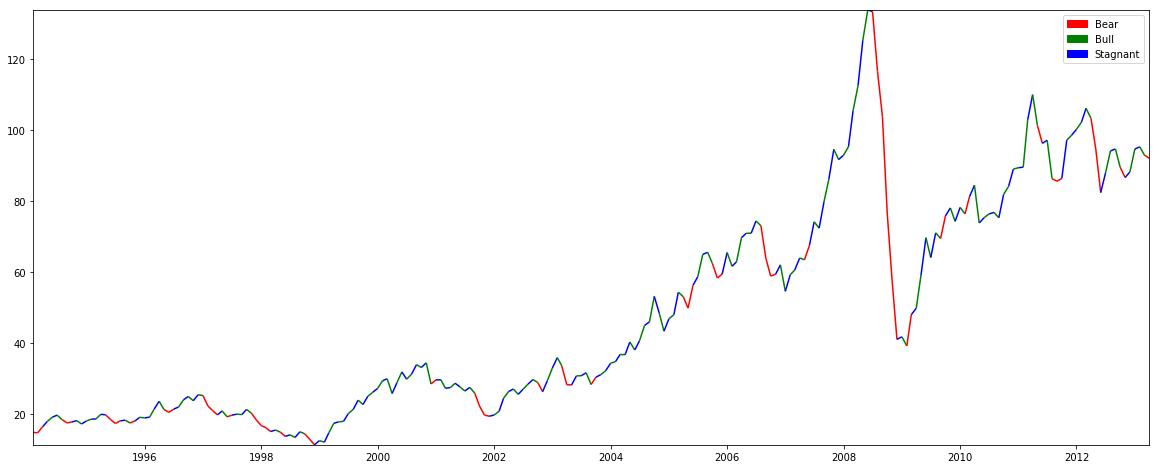
\includegraphics[width=15cm, scale=0.2]{img/index.png}
  \caption{\texttt{hmms} provides a graphical representation of HMMs, illustrating the hidden states and emission states as state and emission sequences.}
\end{figure}

Given that Hidden Markov Models are highly applicable in a number of time-series analysis applications (Barber, D) \cite{barber2011bayesian}, we would be using \texttt{hmms} for analysing financial time-series data obtained from the FRED and EIA. We would be using \texttt{hmms} to identify bull and bear regimes in time-series data in an attempt to discretise our time-series to be used in a Bayesian Network. We would be discussing this in the next \hyperref[regime]{chapter}. \\




\section{Datasets in macroeconomic perspective}

We would be using the \href{https://www.eia.gov/}{Energy Information Administration} (EIA) and the \href{https://fred.stlouisfed.org/}{Federal Reserve Economic Data} (FRED) to retrieve datasets of different macro-economic data to incorporate in our model. Fortunately, both data centres have Python APIs and allow to neatly retrieve data as a \texttt{pandas} dataframes without any messy \texttt{curl} or \texttt{wget} UNIX calls.

\subsection{Physical market factors from EIA}
\label{eia}

The Energy Information Administration (EIA) has a number of datasets for macro-economic inference on the oil markets. Other than by collecting macro-economic data which affects the oil markets, the EIA also assists oil market analysts in constructing statistical models for the oil markets, along with providing an expert knowledge about the relationship between the different macroeconomic variables. \\

In a report compiled by EIA \cite{eiaoilpriceforecasts} \href{http://www-personal.umich.edu/~lkilian/}{Kilian, Lutz}, short-term oil prices have been forecasted using vector autoregression (VAR), spread between oil future prices and oil spot prices, forecasts based on non-oil industrial commodity prices, and the forecasts relying on the time-varying parameter (TVP) model of the spread between U.S. gasoline spot prices and heating oil, and spot price of crude oil.\\

In a study \cite{whatdrivescrudeoilprices} conducted by \href{mailto:bruce.bawks@eia.gov}{Bruce Bawks}, a financial analyst of the Energy Markets at the EIA, it was determined that several macroeconomic factors affect the price of oil and therefore these factors could be used in models for a short-term forecast of oil markets.  The price of oil can be influenced by geopolitical events, such as OPEC and non-OPEC relations, and events resulting in political instability in the Middle East such as the Iran-Iraq War and Iraq's invasion of Kuwait. Market inefficiency \footnotemark in oil markets can allow arbitrage, therefore affecting the price in different markets.  Economic growth has a strong affect on the price of oil (which would be discussed in \hyperref[fred]{FRED} data). Changes in OPEC production, such as unplanned supply disruptions or production quotas, affect the price of oil. Determining every factor which affects the price of oil is unfeasible, given F.A Hayek's notion of that no single agent in the market can determine all factors affecting the price and production in a system \cite{book:642976}.  \\

The relevant macroeconomic data from the EIA is updated at a monthly frequency. This results in a constraint on the time period at which we get predictions on statistical confidence. \href{https://www.linkedin.com/in/delaney-granizo-mackenzie-23965080/}{Delaney Mackenzie} at Quantopian, described what is known as the \enquote{\href{https://twitter.com/thestreetquant/status/959449801321517056}{30x rule of thumb}} \label{30x}, which asserts that if the data is sampled at frequency $f$, we can only achieve statistical confidence at $30f$. So given we have data sampled at a monthly frequency, we only can achieve predictions on a multi-year trend. \\

\footnotetext[1]{Inefficient markets refer to the phenomenon where an asset's market price does not accurately reflect its true value, therefore allowing traders to simultaneously purchase and sell the asset for a profit.}

\subsection{FRED}
\label{fred}

The Federal Reserve Economic Data, St. Louis (FRED) is a collection of  508,000 US and international time series from 86 sources \cite{fredweb} on different macroeconomic data such as the consumer price index, producer price index, and Industrial Production index. Similar to the EIA, the FRED not only provides macroeconomic datasets but also provides expert knowledge about the relationships between different sectors of the economy.  The FRED also provides a lot of expert knowledge about how different macro-economic indicators play a role in determining the price of oil.\\

In a study by Kilan, Lutz study \cite{lutzreport}, a structural decomposition of the real price of crude oil was proposed; the three factors affecting the price of oil were crude oil supply shocks, shocks to the global demand for all industrial commodities, and demand shocks that are specific to the crude oil market. Basing on Kilians study,  Alejandro Badel and Joseph McGillicuddy \cite{badelmcgillicuddy} at the FRED carried out a research, exploring the correlation between the oil prices and inflation expectations, and came up with three conclusions. \\

Firstly, the study concluded the fact that in the entire time frame 2003-2015 there was little correlation between the inflation expectation and oil price, but during the 2007-2008 Financial Crisis there was a high correlation suggests that the financial crisis was some sort of an 'exception' and the level shift in the inflation expectations unrelated to the oil price shocks. Secondly, it concluded that only the correlation of oil-specific demand shocks and inflation expectations was positively significant across all sub-periods (excluding the 2007-2008 Financial Crisis) Thirdly, it suggests that there is a need to investigate the nature of oil specific demand shocks. \\

Similar to the EIA data, the macroeconomic data from the FRED comes at a monthly frequency, rendering our model accurate to multi-year trends (30 months) by the \emph{30x rule of thumb}. In a research conducted by Kilian \cite{hftoil}, it has been concluded that not has been lost by not using high-frequency data, however, given that MIDAS model was used, it might be possible that HMMs are better trained with more high-frequency data.\\

The FRED, just like the EIA fortunately has a (third party) Python API \cite{fredgit} which allows us to retrieve data very, very neatly as a \texttt{pandas} dataframe from the FRED database. Similar to the EIA data, FRED data often has holes, however, the indexes are formatted as \texttt{dates} so thus not much data preprocessing would be needed.\\
